\documentclass{article}
% Copyright 2017 Sergei Tikhomirov, MIT License
% https://github.com/s-tikhomirov/solidity-latex-highlighting/

\usepackage{listings, xcolor}

\definecolor{verylightgray}{rgb}{.97,.97,.97}

\lstdefinelanguage{Solidity}{
	keywords=[1]{anonymous, assembly, assert, balance, break, call, callcode, case, catch, class, constant, continue, constructor, contract, debugger, default, delegatecall, delete, do, else, emit, event, experimental, export, external, false, finally, for, function, gas, if, implements, import, in, indexed, instanceof, interface, internal, is, length, library, log0, log1, log2, log3, log4, memory, modifier, new, payable, pragma, private, protected, public, pure, push, require, return, returns, revert, selfdestruct, send, solidity, storage, struct, suicide, super, switch, then, this, throw, transfer, true, try, typeof, using, value, view, while, with, addmod, ecrecover, keccak256, mulmod, ripemd160, sha256, sha3}, % generic keywords including crypto operations
	keywordstyle=[1]\color{blue}\bfseries,
	keywords=[2]{address, bool, byte, bytes, bytes1, bytes2, bytes3, bytes4, bytes5, bytes6, bytes7, bytes8, bytes9, bytes10, bytes11, bytes12, bytes13, bytes14, bytes15, bytes16, bytes17, bytes18, bytes19, bytes20, bytes21, bytes22, bytes23, bytes24, bytes25, bytes26, bytes27, bytes28, bytes29, bytes30, bytes31, bytes32, enum, int, int8, int16, int24, int32, int40, int48, int56, int64, int72, int80, int88, int96, int104, int112, int120, int128, int136, int144, int152, int160, int168, int176, int184, int192, int200, int208, int216, int224, int232, int240, int248, int256, mapping, string, uint, uint8, uint16, uint24, uint32, uint40, uint48, uint56, uint64, uint72, uint80, uint88, uint96, uint104, uint112, uint120, uint128, uint136, uint144, uint152, uint160, uint168, uint176, uint184, uint192, uint200, uint208, uint216, uint224, uint232, uint240, uint248, uint256, var, void, ether, finney, szabo, wei, days, hours, minutes, seconds, weeks, years},	% types; money and time units
	keywordstyle=[2]\color{teal}\bfseries,
	keywords=[3]{block, blockhash, coinbase, difficulty, gaslimit, number, timestamp, msg, data, gas, sender, sig, value, now, tx, gasprice, origin},	% environment variables
	keywordstyle=[3]\color{violet}\bfseries,
	identifierstyle=\color{black},
	sensitive=false,
	comment=[l]{//},
	morecomment=[s]{/*}{*/},
	commentstyle=\color{gray}\ttfamily,
	stringstyle=\color{red}\ttfamily,
	morestring=[b]',
	morestring=[b]"
}

\lstset{
	language=Solidity,
	backgroundcolor=\color{verylightgray},
	extendedchars=true,
	basicstyle=\footnotesize\ttfamily,
	showstringspaces=false,
	showspaces=false,
	numbers=left,
	numberstyle=\footnotesize,
	numbersep=9pt,
	tabsize=2,
	breaklines=true,
	showtabs=false,
	captionpos=b
}

\usepackage[UTF8]{inputenc}
\usepackage[english]{babel}
\usepackage{float}
\usepackage{csquotes}
\usepackage{amsmath}
\usepackage{listing}
\usepackage{hyperref}
\usepackage{graphicx}
\usepackage[most]{tcolorbox}
\definecolor{block-gray}{gray}{0.85}
\hypersetup{urlbordercolor={white}, linkbordercolor={white}, citebordercolor={white}}
\graphicspath{ {../images/} }
\newtcolorbox{blockqt}{colback=block-gray,boxrule=0pt,boxsep=0pt,breakable}
\title{ \begin{huge}
\textbf{Epress World: A Peer-to-Peer World Community} 
\end{huge} }
\author{ Garbin Huang \\ garbinh@gmail.com \\ epress.world }
\begin{document}
\maketitle
\begin{abstract}
 A purely peer-to-peer information exchange network should allow people to easily send information from one node to another node without going through a centralized server. Personal privacy and data will no longer be  stored on third-party centralized servers and get rid of the dependence on large service providers such as Facebook,Twitter, etc.Getting rid of the dependence on large service providers means people can retrieve the control of their personal data so as to avoid the privacy violations as well as  the threat of potential large-scale data leak. But this can only solve part of the problem. The flood of false misleading 
information and usurpation of digital content are still unavoidable. We propose a solution to this problem using a peer-to-peer information exchange network.The information circulating in the network must be with  an irrevocable proof-of-source. the information receiving node can easily verify the proof-of-source.  Only if the source node of the information is trusted and the proof-of-source is verified,the information can be recieved. the information receiving node will save the copy of the full information,this will be helpful to decrease the false misleading information of the system.In order to solve the problem of digital content misappropriation,we also will implement information right confirmation based on the  the Ethereum blockchain and smart contracts.
\end{abstract}
\section{Introduction}\label{introduction}
    Nowadays, people's digital life cannot be separated from the Internet, digital media and social networks. Relying on them it brings convenience,meanwhile, new challenges too.In order to use the services provided by these digital media and social networks,people had to tranfer their usage rights of their personal data to the provider\cite{twitter_tos}\cite{facebook_tos}. privacy violations are inevitable.At the same time, due to the centralized data storage of the centralized network,once the system suffers malicious attack. a large-scale data leak will do unpredictable harm.In addition, the centralized system lacks a mechanism to effectively deal with false misleading information.\cite{twitter_fakenews}\cite{fb_fakenews}. The malicous attacker can spread false misleading information in the system with multiple anonymous identities without being discovered or punished, which leads to the flood of false misleading information.In terms of community governance, the owners of a centralized system have absolute control,they can delete, block information, or directly disable accounts,but this power may not be used correctly due to the different interest demands, ideologies and political tendencies,this is inevitable,true fairness is actually impossible.Regarding to digital content disappropriation. it is difficult for traditional copyright identification agencies to play a role in the borderless digital world.On the one hand, creators are powerless against digital content misappropriation, and on the other hand, they will also discourage creators' creative enthusiasm. We cannot rely on centralized service providers to build a free and open world community.

    We need a peer-to-peer information exchange network which doesn't rely on third-party centralized servers.This network allows people to exchange the information directly without going through a centralized system.In addition, the information circulating in the network can be traced to the source. On the one hand, the traceable information can help the information receiver to judge the reliability of the information source. on the other hand,people will be more cautious before sending information since the information and its source is irrevocable, and under the combined effect of the two aspects, it is expected to reduce the infringement of false misleading information on the Internet.We also need to realize information right confirmation without relying on traditional copyright identification agencies. By doing this it doesn't only solve the problem of digital content misappropriation, but can also indirectly promote people's high quality content creations in the community because the rights of content creators can be effectively protected.False misleading information is suppressed or reduced, and excellent valuable information is encouraged or increased,all above will benefit everyone in the community.
    In fact, before Epress World, countless organizations and individuals have actively explored these aspects. For example, in order to retrieve the individual's control over personal data, the EU adoptes GDPR.
    \cite{gdpr}.More examples are such as the historical Diaspora\cite{diaspora}. popular Mastodon \cite{mastodon}. as well as Akasha.World \cite{akasha}founded by Mihai Alisie, one of the co-founders of Ethereum.All of them are very outstanding projects. and have made remarkable achievements.Bitcoin's\cite{bitcoin}successful practice and the infrastructure supplied by Ethereum\cite{ethereum}make it possible to realize all of these better.The difference from the network of bitcoin \cite{bitcoin} is. what circulates in the Bitcoin network is a string of numbers representing value but circulates in the Epress world network is colorful information created by people such as  text, audio, image, video, and even arbitrary binary files.Bitcoin is defined as the World Bank, Ethereum is known as the World Computer, Epress World's vision is to become a more ideal World Community.

    In this white paper, we will propose a peer-to-peer information exchange network that uses an irrevocable proof of source (Proof of Source) to achieve the source traceability of the information circulating within the network, and to achieve information right confirmation based on Ethereum smart contracts.The nodes in the network are individual members of the community. The nodes are connected through trust relationships. Information can only be transferred between the nodes that establish a trust connection with each other. The nodes themselves maintain information storage and node security.The security of the node is the cornerstone of the entire network security. As long as we ensure that the node can be operated safely no matter what kind of network environment it is deployed in, the entire network is safe.
\section{Overview}
    \begin{figure}[H]
        \centering
        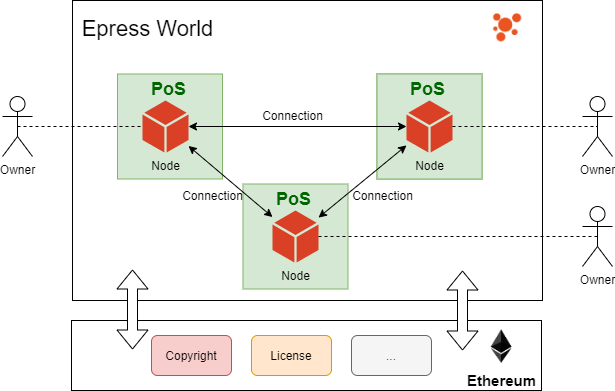
\includegraphics[width=\textwidth]{figures-overview.png}
        \caption{Overview}
    \end{figure}
    As shown in the figure, Epress World is mainly composed of a peer-to-peer information exchange network and Ethereum smart contracts. The peer-to-peer information exchange network is the main body of the Epress World community. The nodes are the information production source of the network. The nodes are connected to each other through trust.The information is allowed to spread within the network under the Proof of Source (PoS) consensus.Ethereum smart contracts give the Epress World community the ability to confirm information rights. Since we hope that people's most information exchange demands can eventually get rid of their dependence on centralized services, the information circulating in the community will be designed to any form, not limited to text, pictures, audio, video, or even any arbitrary  binary files,all of them  will be available in the community.
\section{Implementation of the Network}
    The nodes in the Epress World network correspond to the members of the community, and the nodes will be solely responsible for data storage and security protection.The connection between nodes is established based on trust, and information can be transferred between mutually trusted nodes. In order to realize the source traceability of information, we have proposed the Proof of Source (PoS), and the information needs to be accompanied by a valid proof of source in the circulation process.Node security is the foundation of the entire system security. Epress World's vision is to become an ideal world community. We hope that more people can participate, not just for computer experts.Regardless of age, occupation, and anyone should be able to use it easily and safely. Therefore, we need to ensure that the nodes can still be operated safely and stably under any operating environment and any technical level of management personel,only in this way,the system's security can be ensured.
\subsection{Connection and Trust}
    Establishing a connection between nodes means trust in the Epress World network. The connection can be one-way or two-way.When a node creates a connection to another node, it is equivalent to the node trusting access from another node.When two nodes have added a connection to each other, a two-way connection is established, which indicates that the two nodes trust each other and accept each other's visits and information updates.Ethereum and ECDSA asymmetric encryption algorithms provide us with the cornerstone to build this trust.

    \begin{figure}[H]
        \centering
        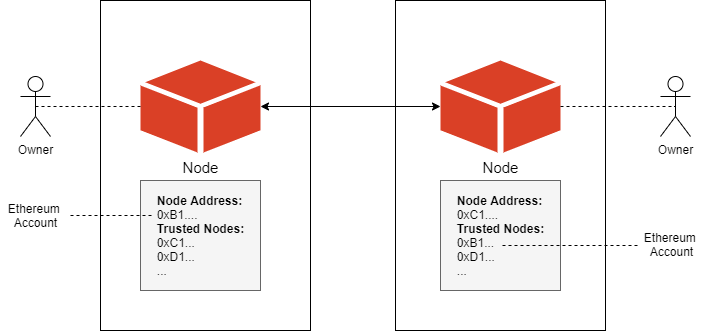
\includegraphics[width=\textwidth]{figures-connect.png}
        \caption{Connection}
    \end{figure}

    As shown in the figure, we can use the Ethereum account address as the identity of the node in the Epress World network, and establishing a connection with other nodes is equivalent to adding the Ethereum address of the other node as a trusted address in its node database.
    ~\newline
    \begin{blockqt}
    \textbf{For example: }Alice decides to establish a connection with Bob, so she adds a connection to the Bob's node on her own node,this means that Alice trust Bob,Bob can visit Alice's node and obtain all her released public information. and if Bob adds a connection to Alice too,the two-way connection between Bob and Alice will be completely bulit,Bob and Alice will be able to obtain the latest updates released by each other through their respective nodes, just like getting the latest Tweet from Following on Twitter, or the latest Feed from Friend on Facebook.
    \end{blockqt}

    Connections can be either established or disconnected freely. Disconnecting is equivalent to losing trust between nodes. The actively disconnected party will reject all access requests and information updates from the passive disconnected party.
\subsection{Information Transfer and PoS consensus}\label{msg_and_pos}
    Information cannot be transferred between nodes untill a two-way connection (that is a two-way trust relationship) is established between nodes.Meanwhile,PoS consensus should be complied with during the information transfer,when sending information,the information from the sending node must be accompanied with proof-of-source,the receiving node will verify the Proof-of-source when receiving the information.The information is received only when the source certificate is verified valid,otherwise,the information will be discarded as unreliable information.See as the following picture: 

    \begin{figure}[H]
        \centering
        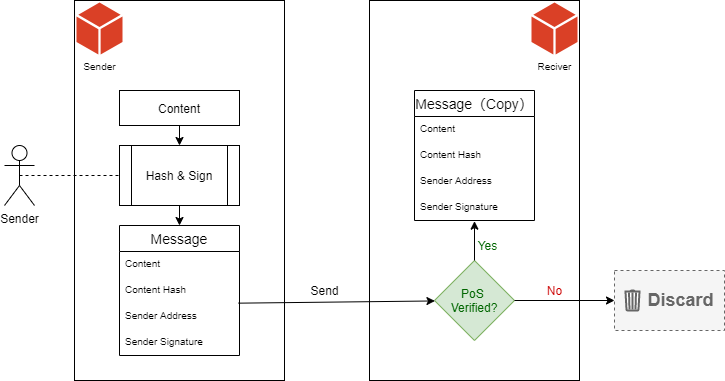
\includegraphics[width=\textwidth]{figures-pos.png}
        \caption{Send Message \& Proof of Source}
    \end{figure}

    Since we have established a trust relationship between nodes based on the Ethereum account system before sending the information, the nodes store each other's Ethereum addresses, and the process of verifying the PoS consensus becomes very simple.First, the information sending node obtains the digest of the information to be sent through the Secure Hash Algorithm(SHA3). The information sender signs the digest through the Ethereum account, and then the Ethereum address, the original information to be sent, the digest and the Ethereum signature will all be packaged and  sent to the information receiving node.After receiving the information, the information receiving node can verify the proof-of-source very simply. If the proof-of-source verification fails, the information receiving node can treat this information as unreliable information and discard it directly.
    ~\newline
    \begin{blockqt}
    \textbf{For example: }Alice(0xB18B7F54eCaD50f22f887702cA2Cd385C5a5332B) and Bob(x50cBF0471AF07Fd2B4Ee30A5BcE2814Ab2cDe4E0) have built a two-way connection. Alice posts a new text update,the content as follow: 
    
    \begin{lstlisting}[caption=Message from Alice, numbers=none]
Hello! Bob.
    \end{lstlisting}
    The digest obtained through SHA3 is:
    \begin{lstlisting}[caption=SHA3 digest of message, numbers=none, breaklines=true]
0x95251fb76809989bd336326b47954b67a02143e913ce0213bfa26
262dc62f4c3
    \end{lstlisting}
    Alice signs the digest with her Ethereum account:
    \begin{lstlisting}[caption=Signature, numbers=none]
0x70b8057ad8984afc1ddf03b521ed45d56a8ee667eff2be7897f45b
a2475f3d655101623b28a1cb8287dac5ec9b5fc1b73697c0304753ad
13f3576e6b3a146b981b
    \end{lstlisting}
    The Alice  node packages this group of information and sends it to the Bob node. After receiving the information, the Bob node verifies whether the content matches with the SHA3 digest to prevent the information from being tampered with during the information transfer, and then verifies whether the signature of the digest comes from Alice's ethereum address.If the verification is passed, the source proves to be valid. The Bob node receives the information and saves a full copy. Alice and Bob complete a typical information transfer.
    \end{blockqt}
\subsection{Group Node}\label{group_node}
    The traditional Internet community does not strictly require only people who have established a trusting relationship can exchange information. On the contrary, the Internet was born to encourage information sharing.For example, on Twitter, anyone can create an account, and anyone can follow accounts of interest. Once the Follow is successful, the followed can broadcast information to hundreds of millions of people around the world at the same time.Although this open method of information transmission has aggravated the spread of false misleading information to a certain extent, it also has its positive side-it expands people's information sources. In addition to trusted people, information can also be obtained from countless strangers.

    In fact, people's information sources cannot only rely on nodes that have established trust connections. Communication with strangers, and obtaining important information from strange nodes is also a very important part of people's current digital life.Group nodes will become a bridge for information exchange between people and strangers.Although we cannot directly establish two-way connections with unfamiliar nodes, we can establish indirect connections through intermediary nodes that both parties trust. We define such intermediary nodes as Group nodes.As the following picture shows:

    \begin{figure}[H]
        \centering
        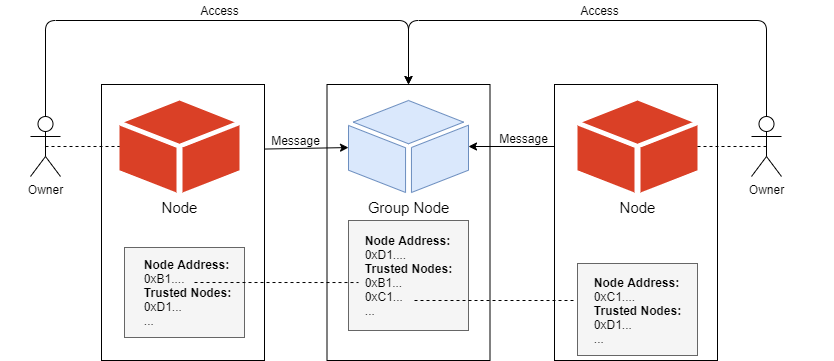
\includegraphics[width=\textwidth]{figures-group.png}
        \caption{Group}
    \end{figure}
    
    The Group node has established  direct two-way connections with both parties. Therefore, either party can directly send information updates to the Group node, and because the group node will save a full copy of the information, the other party in the relationship will be able to access the Group node to obtain the party's release update information,the information exchange between unfamiliar nodes is realized.
    \newline
    \begin{blockqt}
    \textbf{For example: }Alice and Carol are strangers to each other. They are both Bitcoin enthusiast. They cannot exchange information before Alice and Carol know each other and establish a two-way connection.Fortunately, Isaac is an enthusiastic Bitcoin enthusiast. He established a Group node called Bitcoin Group in Epress World. Anyone can self-help to complete the two-way connection to the Bitcoin Group node.Both Alice and Carol have established a two-way connection to the Bitcoin Group, so they can both send all the information they want to share with other Bitcoin enthusiasts to the Bitcoin Group.Carol wrote an excellent Bitcoin protocol improvement article, and sent the signature of the article to the Bitcoin Group node. Alice saw this article signed by Carol by visiting the Bitcoin Group node. Alice knew  Carol through the Bitcoin Group channel and got a great article about Bitcoin Improvement Protocol written by a stranger here.
    \end{blockqt}
\subsection{System Security}
    Node security is the foundation of the security of the entire Epress World network system. We need to ensure that anyone can safely and stably run their respective nodes in as many environments as possible. Epress World nodes will be designed to be used in professional computer rooms,small home servers,NAS, personal PC desktops, laptops, even mobile phones.Therefore, we need to make sure the node  is safe even if it is running on a home network without professional network protection conditions and management personnel. We will explain how we can achieve this goal from two perspectives: data security and node instance security
\subsubsection{Data Security}
    In the absence of professional network protection and management personnel, we should assume that the probability of any node being invaded by a malicious attacker is 100\%. We need to ensure that after the node is invaded, the sensitive data won't be leaked, and the attacker cannot send information with the identity of the compromised node falsely.

    Thanks to the distributed account design of Ethereum, we can use the Ethereum account as the identity of the node, and realize identity authentication through signature, so it's not necessary for the node to store identity authentication information such as passwords and private keys.In this way, even if the attacker invades and obtains the full control authority of the server where the node is located, he cannot obtain the private key of the node's Ethereum account, and cannot provide a valid digital signature, and moreover, the information transmission in the network is restricted by the PoS consensus, he cannot send any information with the identity of the compromised node.

    \begin{figure}[H]
        \centering
        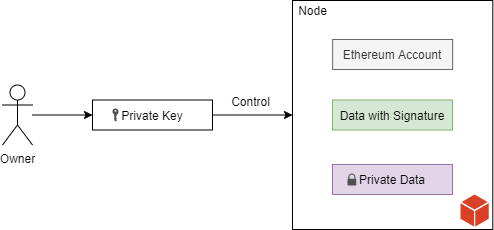
\includegraphics[scale=0.6]{figures-data_security.png}
        \caption{Data Security}
    \end{figure}

    In the Epress World network, the full and irrevocable copy of the information with proof of source will be kept  by all receiving nodes. Therefore, we will define the information with proof of source as public information. Since this information is irrevocable and may be made public sooner or later,the possible harm caused by the attacker's intrusion is limited.But people also have the demand to store private information. For private information, we can use a symmetric encryption algorithm such as AES256 to encrypt the content and store the password offline.In this way, even if an attacker invades, he cannot obtain private information in plain text.
    ~\newline
    \begin{blockqt}
    \textbf{For example: }Alice's node was invaded by a malicious attacker Mallory. After Mallory invaded, he wanted to use Alice's identity to send false text updates to all of Alice's friends. He wanted  Alice's friends to  transfer money to Mallroy's Bitcoin address, and Mallory obtained the full access to the server and database of Alice's node. He added the false information that he wanted to obtain the bitcoin transfer into the node's database. Due to the PoS consensus of information transfer between nodes, the text information cannot be received by other nodes until the signature enclosed with the text is matched with the signature of the node's corresponding Ethereum account.And because Alice's Ethereum wallet is not stored on the node server, Mallory cannot obtain the right digital signature to make the text information with matched signature.Even if he can successfully write this information into Alice's node database, this updated text can't be received by Alice's friends,because the information without a valid proof-of-source cannot be spreaded within the Epress World network.Besides, because Alice is careful to encrypt all private data, Mallory cannot view all the private information that Alice saves in the node. 
    \end{blockqt}
\subsubsection{Instance Security}
    The node instance runs in a network environment without a professional network firewall.It is extremely vulnerable to be attacked such as DDoS and cause the node server paralyzed.This will affect the node's normal participation in the Epress World community.And if people run the node in a network environment that lacks effective protection, malicious attackers will easily force people to be unable to use the node.We had to ensure that people can respond effectively to this threat.

    \begin{figure}[H]
        \centering
        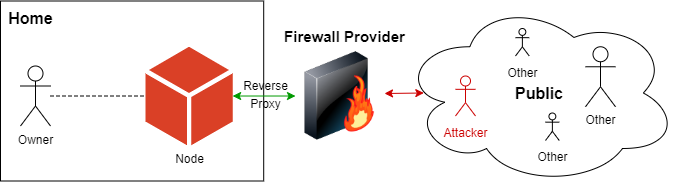
\includegraphics[width=\textwidth]{figures-firewall.png}
        \caption{Firewall}
    \end{figure}

    As shown in the figure, we assume that the nodes are deployed in a home network that lacks effective protection. In order to ensure the safety of these nodes, we can provide safe and reliable network egress services for these nodes through a reverse proxy in a computer room with professional protection conditions.Just like the services provided by Amazon CloudFront and Cloudflare, this is actually a very mature technology and industry.
\section{Blockchain and Copyright}
    In the traditional network community, there is a lack of independent and impartial copyright identification agencies to provide ownership confirmation services for people's digital content, this makes it difficult for people to claim their ownership of original content. In the face of the information theft, content owners can do nothing but report to major platforms.If your content is recognized by copyright organizations in reality, you may be able to smoothly punish the pirates. For the globalized world community, such rights protection costs are high and not friendly to people's daily creation.

    The non-tamperable feature of the Ethereum blockchain and open smart contracts can help us confirm information rights.Through smart contracts, we can write the information and proof of source (digital signature) as the owner's proof of ownership into the public Ethereum blockchain database, thus information right confirmation is realized.


    \begin{figure}[H]
        \centering
        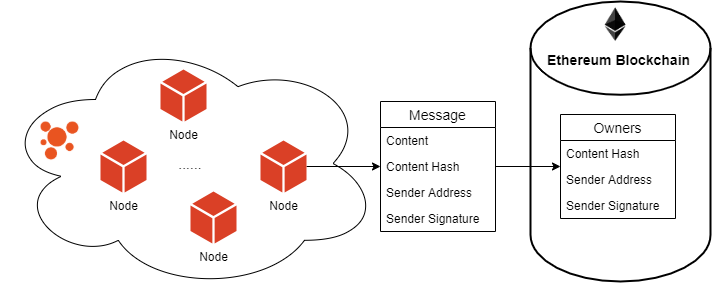
\includegraphics[width=\textwidth]{figures-blockchain.png}
        \caption{Ethereum Blockchain}
    \end{figure}
    
    In the chapter \ref{msg_and_pos} we mentioned the circulation of information in the Epress World network, which contains the Content Hash value (Checksum) that prevents tampering during the transmission process. When the content changes, the Content Hash will also change.The different information always has a different Content Hash, just like the fingerprint of the data.It is expensive and unrealistic to store full information content in the Ethereum blockchain, so we can write this value as a content equivalent into the blockchain database.
    As shown in the figure, the nodes in Epress World send the generated information , the corresponding Hash, the creator's Ethereum address and the signature corresponding to the content to the Epress World contract.The contract verifies whether the Hash has been recorded (whether it has been registered of ownership preemptively by others), then the contract verifies whether the signature corresponding to the Hash matches that of the sender for the transaction.If the verification is passed, the information confirmation registration is completed. In this way, people can prove that they are the owner of the content through the information in the Ethereum blockchain.
    ~\newline
    \begin{blockqt}
    \textbf{For example: }Both Alice and Charlie are members of the Epress World community and have not known each other before. Alice published a paper on Bitcoin's improved protocol. Alice did not want to use an open authorization protocol to share freely, so she registered it on the Ethereum blockchain first to complete the confirmation of rights,and then Alice posted the paper to the Group node of Bitcoin Group to discuss it with many Bitcoin enthusiasts.Charlie discovered this great paper through Bitcoin Group, and then he copied the original text, without a signature of Alice, and also posted it on his personal Github account in his own name. He has gained great influence on Github because of this great paper. A month later, Alice found this paper on Github. Then she started negotiations with both Charlie and Github. Charlie refused to admit that he misappropriated Alice's paper. Github needed evidence to determine whether Charlie indeed misappropriated Alice's paper for further processing.At this time, Alice showed the block with the copyrights that she registered for the information on the Ethereum blockchain.The block that packaged for this transaction contains time stamp information,and this information cannot be tampered with or forged. Through comparison, it is found that the timestamp information of Alice's confirmation exchange in the block is indeed earlier than the release time of Charlie on Github. At this point, Github can determine that Charlie did misappropriate Alice's paper. With clear evidence, Github handled Charlie's misappropriation. Alice made this negotiation successful because of the first information confirmation for the transaction.
    \end{blockqt}
\section{Community Governance}
    Traditional centralized community service providers usually belong to individuals or commercial companies, and they have control over all resources of the community from software to user data.Theoretically,they can view, modify, delete, and block any user's data at any time without the user's knowledge.They can also temporarily or permanently disable any user's account at any time. Exactly,this is a condition for people to use their services. Such as the user terms of service for Twitter\cite{twitter_tos} and Facebook\cite{facebook_tos}. On this basis, they usually make community rules, and people will be punished by messages being blocked or accounts being disabled etc. when they break the rules. This kind of governance is usually efficient and non-controversial in small centralized communities, but for globalized world communities, this kind of community governance has obvious drawbacks.First of all, in terms of rulemaking, community owners usually have certain ideological and political inclinations out of their own interests or the interests of the country where they are located. On the other hand, in terms of rule enforcement, there will be a certain misjudgment rate for whether people are in violation of the rules or not ,no matter it is judged by machines or manually. Complete fairness and justice is actually impossible to achieve, so there will always be some persons to suffer undue punishment because of misjudging.

    We believe that the real world community should be free and open.Anyone can join or leave the community at any time and there should not be anyone who has the right to allow or prohibit others to participate in the community.There should be no artificial rules of community behavior to constrain people's information creation. People's influence should depend on their accumulating words and deeds. The spread of information should depend on the information itself and should not be interfered by the community's rules.
    
    \begin{figure}[H]
        \centering
        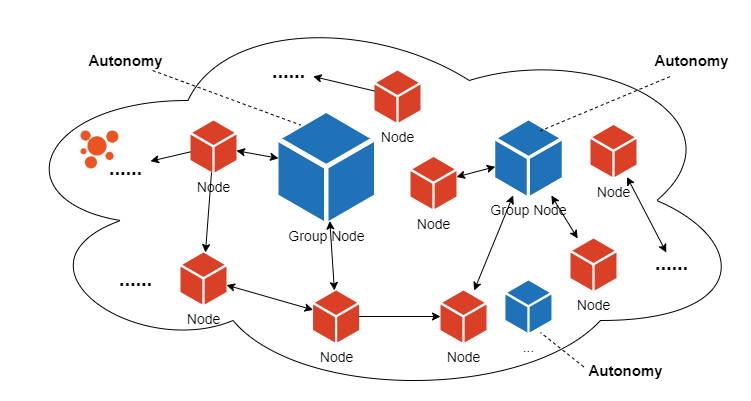
\includegraphics[width=\textwidth]{figures-governance.png}
        \caption{Community Governance Landscape}
    \end{figure}

    As shown in the figure is the panorama of community governance of Epress World.The decentralized system architecture design allows a free and open world community to be realized. Anyone can join or leave the community at any time, and people's information creation does not need to be restricted by any community rules.The dissemination of information will not be subject to any community rules and human interference. As long as the information is welcomed by people, they will be widely disseminated. On the contrary, if the information disgusts people, it may only exist in the information publisher's own node.
    
    Anyone can create Group nodes to realize group communication.The Group node is a small centralized community. For the node owner, there may be both acquaintances and strangers using the node to communicate.In order to maintain order, like most centralized communities, the owners will make community rules.Anyone who uses the Group node to provide services has the obligation to abide by the rules of the node's community.This kind of regional autonomy is also an important part of Epress World community governance.
\section{Conclusion}
    We have proposed a solution to build a world community without relying on centralized servers.Starting from a peer-to-peer information exchange network, the node instances and data are managed and maintained by the community members themselves.They retrieve ownership of personal data in this way to avoid privacy violations and possible threats from large-scale data leak.Then, we realized the trust interconnection between nodes through Ethereum and its signature mechanism, making it possible to exchange information between nodes.Immediately afterwards, we introduced PoS consensus to achieve information source traceability to help improve the quality of information in the community, and made communication between strange nodes possible by introducing Group nodes. Finally, we use the Ethereum blockchain and its smart contracts to confirm information rights to help people solve the problem of digital content theft.

    We hope that Epress World will finally allow people to completely get rid of their dependence on various current centralized communities, regardless of skin color, race, nationality, so that everyone is free from information spam,and benefits from free, equal and efficient information exchange.Thereby,a more ideal world community is realized, benefitting everyone.
\begin{thebibliography}{9}

\bibitem{twitter_tos} 
Twitter Inc.
\textit{Terms of Service}.
\url{https://twitter.com/en/tos}.

\bibitem{facebook_tos} 
Facebook
\textit{Terms of Service}.
\url{https://www.facebook.com/terms.php}.

\bibitem{twitter_fakenews} 
NBC News.
\textit{Twitter is testing new ways to fight misinformation — including a community-based points system}.
\url{https://nbcnews.to/2Vikbfe}, 2020.

\bibitem{fb_fakenews} 
Wired.
\textit{Facebook Is Changing News Feed (Again) to Stop Fake News}.
\url{https://bit.ly/3ebCPhv}, 2019.

\bibitem{gdpr} 
European Parliament, Council of the European Union.
\textit{General Data Protection Regulation}.
\url{https://gdpr-info.eu/}, 2016.

\bibitem{diaspora} 
Diaspora Foundation
\textit{The online social world where you are in control}.
\url{https://diasporafoundation.org/}.

\bibitem{mastodon} 
Mastodon
\textit{Giving social networking back to you}.
\url{https://joinmastodon.org/}.

\bibitem{akasha} 
Mihai Alisie.
\textit{Akasha World}.
\url{https://akasha.org/blog/2017/11/14/new-horizons}, 2017.

\bibitem{bitcoin} 
Satoshi Nakamoto.
\textit{Bitcoin: A Peer-to-Peer Electronic Cash System}. 
\url{https://bitcoin.org/bitcoin.pdf}, 2008.

\bibitem{ethereum} 
Vitalik Buterin.
\textit{A Next-Generation Smart Contract and Decentralized Application Platform}.
\url{https://github.com/ethereum/wiki/wiki/White-Paper}, 2015.

\end{thebibliography}
\end{document} 